\section{扩展板说明}
为了方便把常用器件、外设的引脚集中在一起,制作了一个扩展板,直接插在野火开发板的针脚上,
需要时直接把器件用排线连接到板上即可。

引出接口:

\begin{table}[H]
\center
\begin{tabular}{cccc}
    \hline
    外设 & 引脚数 & 个数 & 使用资源\\
    \hline
    AD9854    & 24  & 1 & GPIO$\times$19
    \tablefootnote{注:其中A0$\sim$A5、D0$\sim$D7 分别需要分配到连续的6个、8个GPIO口上}\\
    AD9910    & 26  & 1 & SPI3/GPIO$\times$16
    \tablefootnote{注:其中PF0$\sim$PF2 需要分配到连续的3个GPIO口上}\\
    ADS124S08 & 7   & 1 & SPI1/GPIO$\times$4 \\
    SPI1      & 4   & 2 & GPIO$\times$1 \\
    SPI2      & 4   & 2 & GPIO$\times$1 \\
    SPI3      & 4   & 2 & GPIO$\times$1 \\
    \hline
\end{tabular}
\captionof{table}{引出接口清单}
\end{table}

下图是扩展板的具体引脚分配(矢量图可放大):

\begin{figure}[H]
\center
    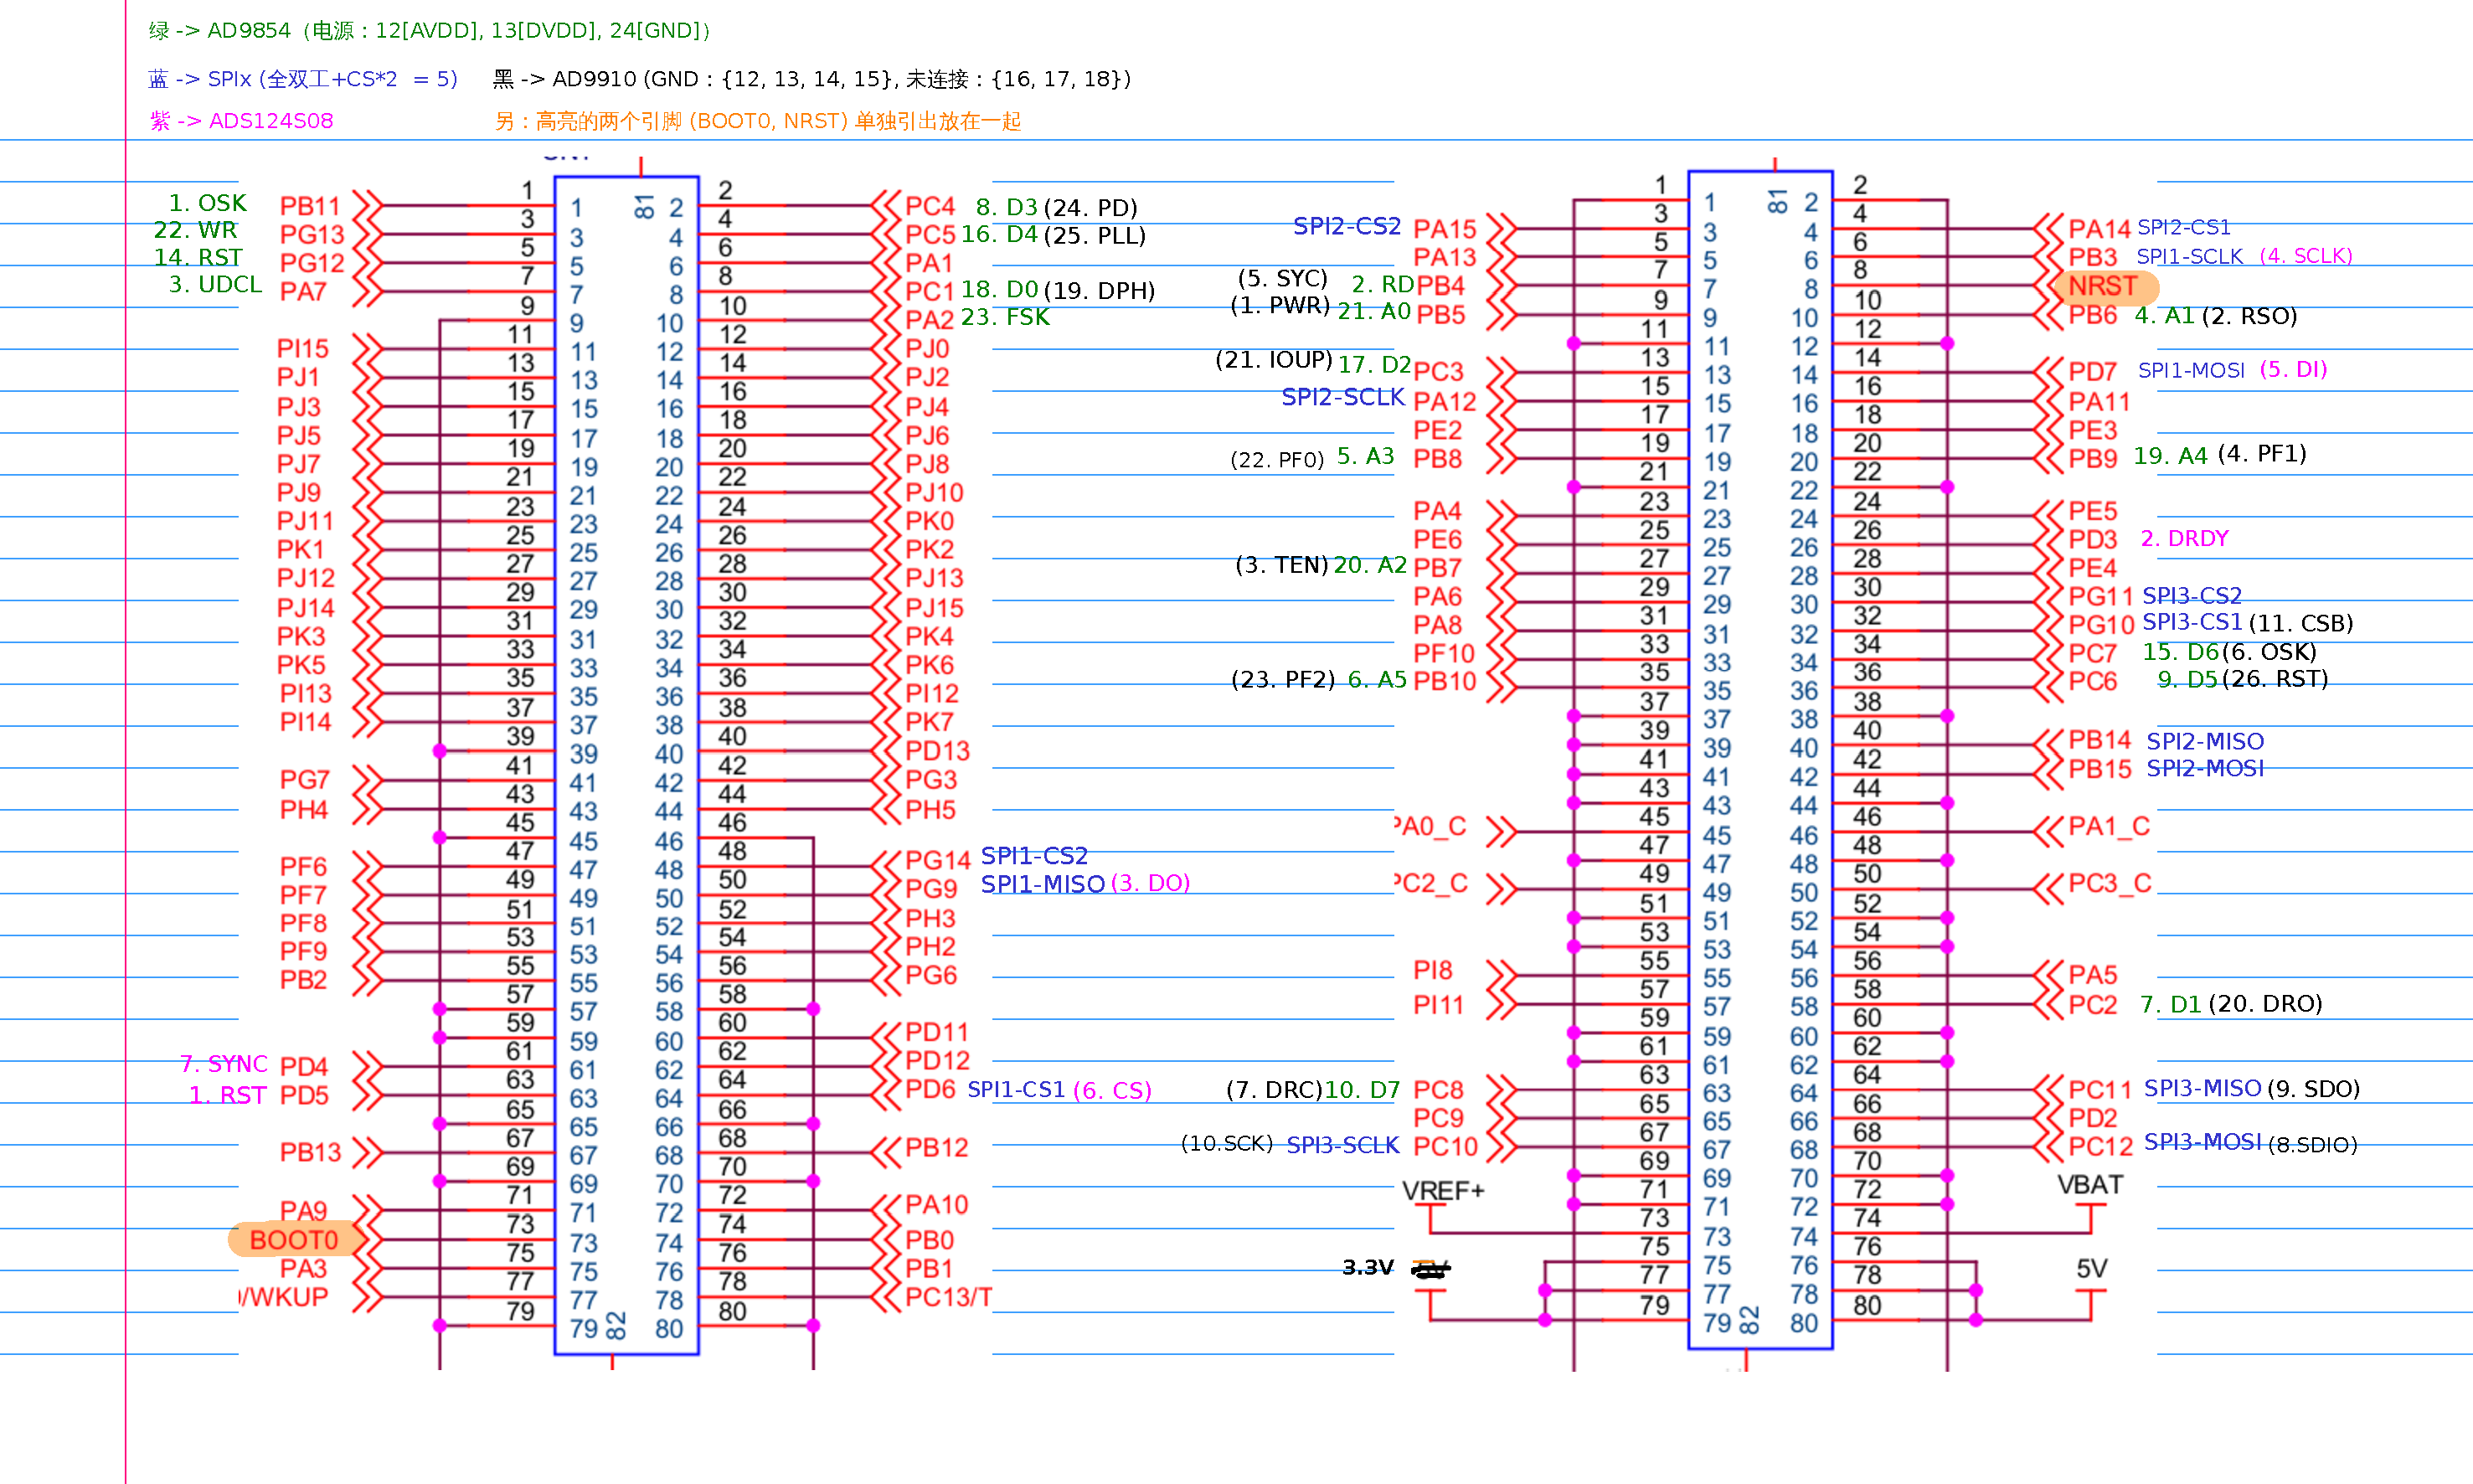
\includegraphics[width=0.8\textwidth]{../扩展板引脚分配图.pdf}
    \captionof{figure}{扩展板引脚分配图}
\end{figure}

其中AD9854、AD9910两个器件使用了双排线来与扩展板连接,其引脚编号(即具体引脚前面的数字)
按照如下约定进行分配:

\begin{displayquote}
在器件正面俯视图的基础上,如排针已是横向排列的,则从左上角开始编号为1,按顺时针增加;
如排针是纵向排列的,则顺时针旋转$90^\circ$后按前述规则编号。
\end{displayquote}

例如,AD9910的引脚编号如下:

\begin{figure}[H]
\center
    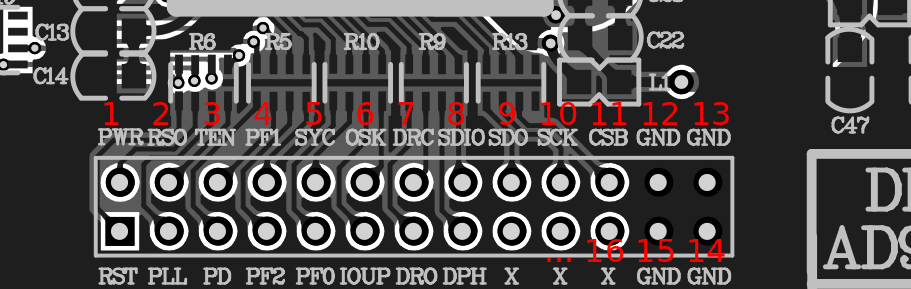
\includegraphics[width=0.8\textwidth]{img/ad9910-pins.png}
    \captionof{figure}{AD9910 PCB板}
\end{figure}
